\chapter{Primeri uporabe}



\section{Napoved temperature s pomočjo CO2 emisij v ZDA}



postavitev kaze slika \ref{co2_temp_indicator}

\begin{figure}
\begin{center}
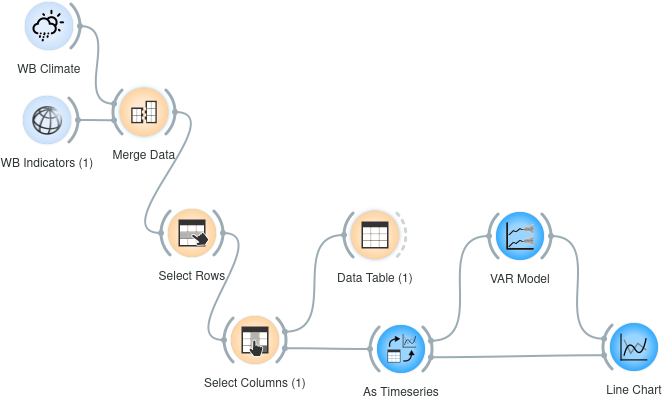
\includegraphics[width=11cm]{pic/var_setup.png}
\end{center}
\caption{Prikaz povezave gradnikov za napoved temperature.}
\label{co2_temp_forecast}
\end{figure} 


\begin{figure}
\begin{center}
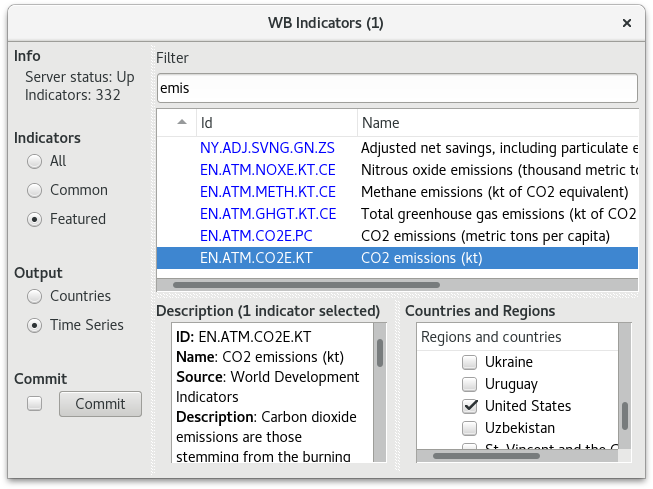
\includegraphics[width=12cm]{pic/var_indicator_select.png}
\end{center}
\caption{Izbor indikatorja CO2 emisij v ZDA.}
\label{co2_temp_setup}
\end{figure} 

\begin{figure}
\begin{center}
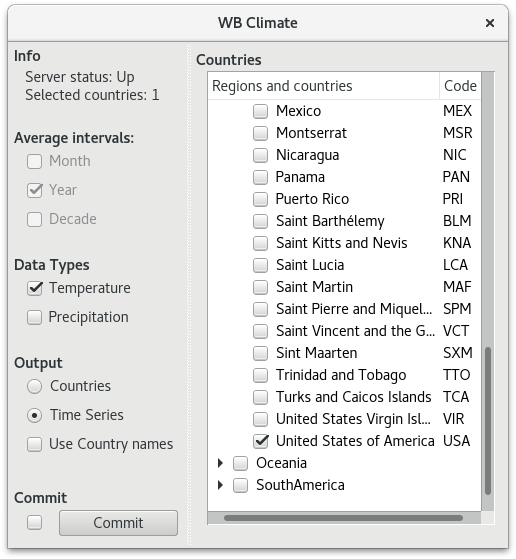
\includegraphics[width=8cm]{pic/var_climate_select.png}
\end{center}
\caption{Izbor podatkov povprečnih letnih temperatur v ZDA.}
\label{co2_temp_forecast}
\end{figure} 

\begin{figure}
\begin{center}
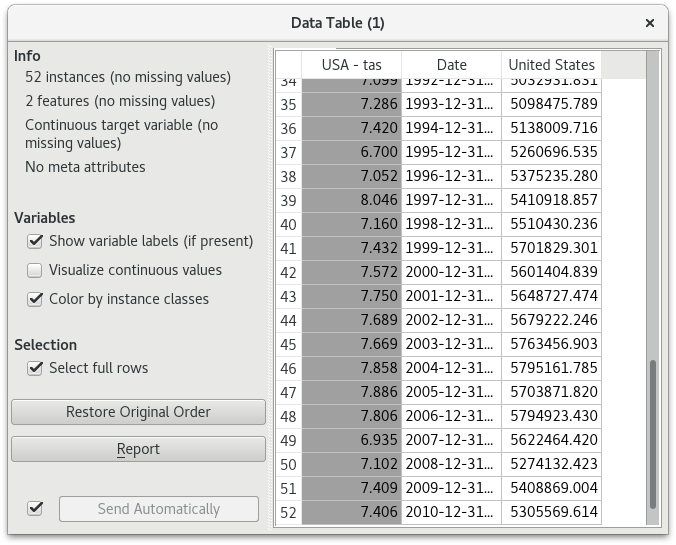
\includegraphics[width=10cm]{pic/var_data_table.png}
\end{center}
\caption{Prikaz združenih podatkov indikatorjev in podnebnih meritev.}
\label{co2_temp_forecast}
\end{figure} 

\begin{figure}
\begin{center}
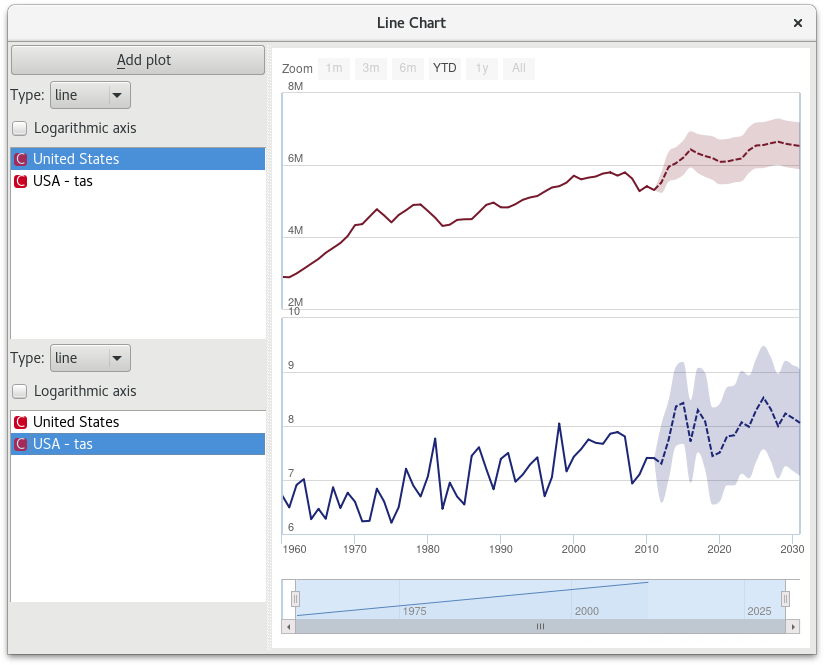
\includegraphics[width=12cm]{pic/var_forecast_graph.png}
\end{center}
\caption{Prikaz napovedi gibanja povprečnih letnih temperatur in emisij CO2.}
\label{co2_temp_forecast}
\end{figure} 




\section{Clustering drzav }



\begin{figure}
\begin{center}
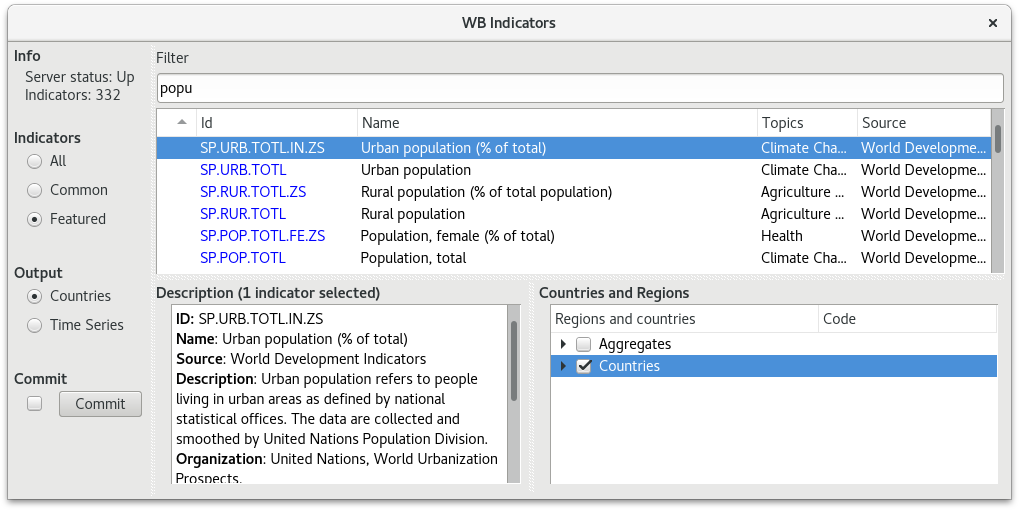
\includegraphics[width=12cm]{pic/cluster_indicators.png}
\end{center}
\caption{Izbor indikatorjev za clustering.}
\label{cluster_indicators}
\end{figure} 

\begin{figure}
\begin{center}
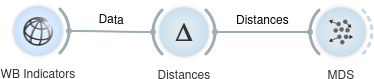
\includegraphics[width=5cm]{pic/cluster_setup.png}
\end{center}
\caption{Postavitev okalja za MDS clustering.}
\label{cluster_indicators}
\end{figure} 

\begin{figure}
\begin{center}
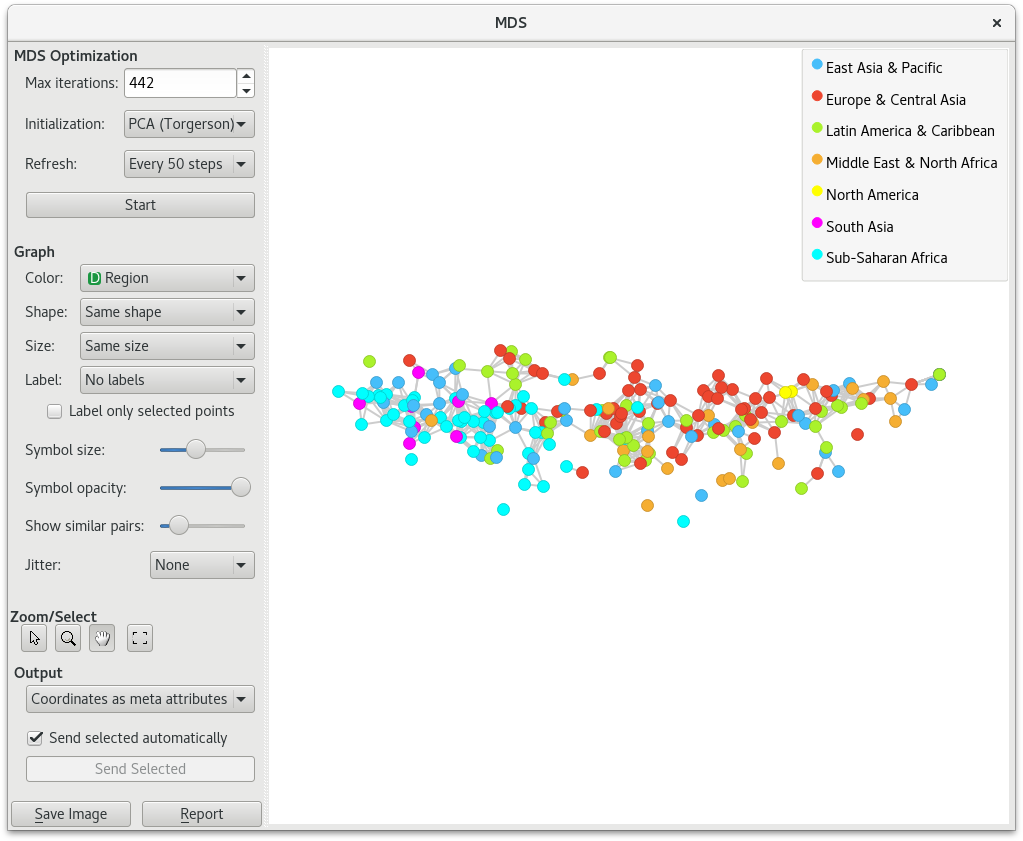
\includegraphics[width=12cm]{pic/cluster_mds_result.png}
\end{center}
\caption{Rezutat MDS clusteringa.}
\label{cluster_indicators}
\end{figure} 
